\chapter{Optimized Waypoints Selection} \label{chap:optimizedway}


%%%%%%%%%%%%%%%%%%%%%%%%%%%%%%%%%%%%%%%%%%%%%%%%%%%%%%%%%%%%%%%%%%%%%%%%%%%%
%%%%%%%%%%%%%%%%%%%%%%%%coverage%%%%%%%%%%%%%%%%%%%%%%%%%%%%%%%%%%%%%%%%%%%%
%%%%%%%%%%%%%%%%%%%%%%%%%%%%%%%%%%%%%%%%%%%%%%%%%%%%%%%%%%%%%%%%%%%%%%%%%%%%
\section{Coverage}

\subsection {Context of experiment}

The main purpose of our work is to estimate the position of $n$ camera waypoints for surveying a given area in order to maximize the visual coverage. Each camera provides a top view of the area similar to UAV views. The coverage area of each camera is defined by the projection of the visual field onto the ground. This way, the mosaic composed of the captured images should be very close to a complete top view of the area. 
In order to find the best coverage, many experiments have been done to compare PSO and also GA. PSO is easier to implement and runs faster but GA is more flexible and generic thanks to the many tunable parameters. 
The following subsections will give an  overview our method, which is based on GA, and provide a comparison between PSO and GA that demonstrates the overall advantage of the latter on the former.

\subsection{ Cost function }

Since the goal is to maximize the visual coverage of the camera network, a cost function has been chosen to quantify it, as follows: 
\begin{equation}
 \sum_{i=1}^n = \frac{cover(i)}{size(grid)} _{1\leq i\leq n}  ,
\end{equation}
where $n$ is the number of waypoints; 
$grid$ represents the discretization of the ground plane (floor);
$cover($ ... $)$ is a function which computes the area on the ground which is covered by at least one camera ;
$size($...$)$ is the dimension of the full area which must be $covered (grid)$. 
% \begin{itemize}
% \item[-] Where $n$ is the number of cameras; 
% \item[-] $grid$ represents the discretization of the ground plane (floor);
% \item[-] $cover(…)$ is a function which computes the area on the ground which is covered by at least one camera ; %(see the pseudo-code below);
% \item[-] $size(…)$ is the dimension of the full area which must be $covered (grid)$. 
% \end{itemize}



\begin{figure}[!htb]
\minipage{0.40\textwidth}
  \includegraphics[width=\linewidth]{figures/Camera.jpg}
  \caption{Projection of the camera on the ground.}\label{fig:cam_proj}
  \endminipage\hfill
\end{figure}

Camera projection model is not explicitly taken into account, but the ground-projected visual field instead, as described in Fig.\ref{fig:cam_proj}.

%\includegraphics[width=0.3\textwidth]{Camera.jpg}
%\caption{Projection of the camera on the ground}
\subsection{Genetic algorithm }
Motivated by Darwin's theory of evolution and the concept of “survival of the fittest”, GAs use processes analogous to genetic recombination and mutation to promote the evolution of a population that best satisfies a predefined goal [12]. Such kind of algorithms requires the definition of a “genetic representation” of the problem and of a cost function used to evaluate the solution. The candidate solution is represented by a data structure named chromosome, defined by Eq.(\ref{Eq:xyzteta}) with $x,y$ and $z$ the cartesian coordinates and $\theta$ the rotation of the camera with respect to the optical axis: only  two possible angles are allowed, 0$^{\circ}$  or 90$^{\circ}$ (portrait or landscape). To pass from an iteration (or generation) to the other a few steps are necessary (see Fig.\ref{fig:GAexp}).
\begin{equation}\label{Eq:xyzteta}
     A=\begin{bmatrix}
         X_{i} \\
         Y_{i} \\
         Z_{i}\\
         \theta_{i}
        \end{bmatrix}_{1 \leq i \leq n}
  \end{equation}

\begin{figure}[t]
\minipage{0.95\textwidth}
  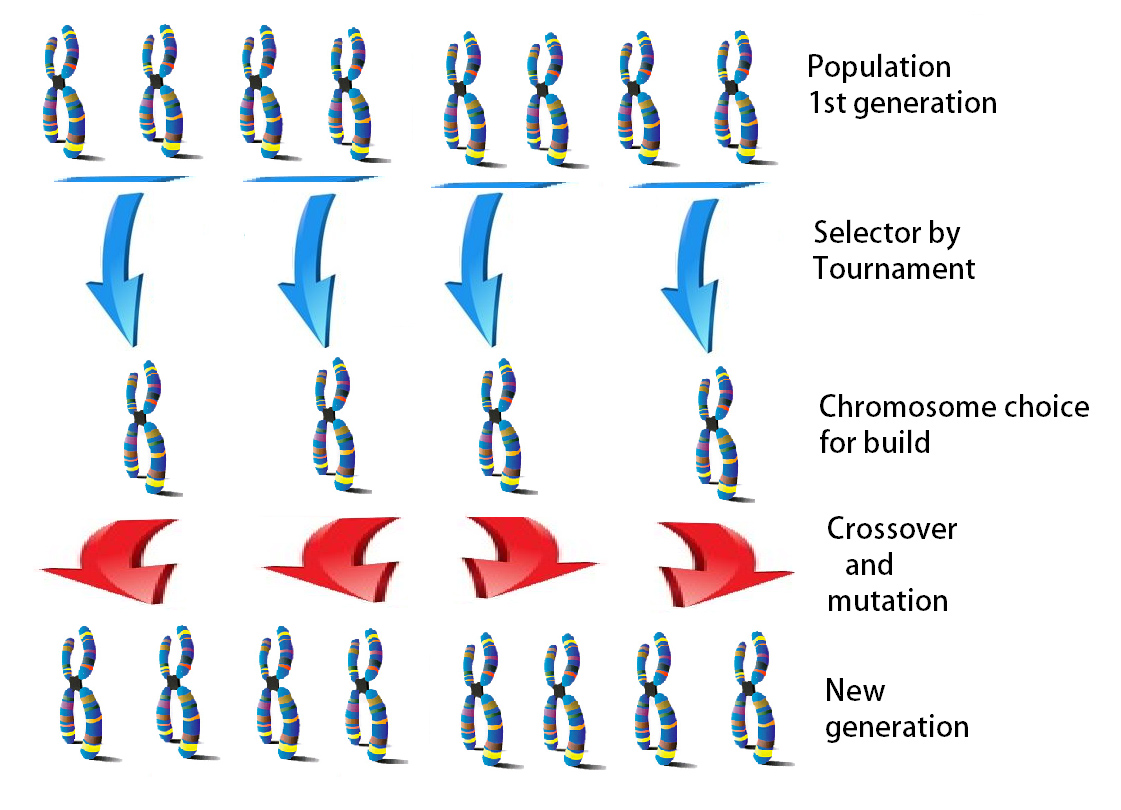
\includegraphics[width=\linewidth]{figures/GAfinal.jpg}
  \caption{ GA explanation, from one generation to the other.}\label{fig:GAexp}
  \endminipage\hfill
\end{figure}
In our experiments, we empirically fixed %after having sevral test in difrent condition the solution shosen is
the number of chromosomes to be 90, the mutation rate to be 0.001 and the crossover rate to be 0.919. 

\subsection{ Context of experimentation }

In order to compare the two algorithms and evaluate their performances, we tested them on different scenarios depicted in Fig.\ref{fig:Rooms_shapes}, with areas  of different sizes and shapes, where: 

\begin{figure}[!htb]
  \centering
  \hspace*{\fill}
  \subfigure[]{\label{subfig:r1}\includegraphics[width=0.45\linewidth]{figures/Room1.png}} \hfill
  \subfigure[]{\label{subfig:r3}\includegraphics[width=0.45\linewidth]{figures/room3.png}}
  \hspace*{\fill}
  \\
  \hspace*{\fill}
  \subfigure[]{\label{subfig:r2}\includegraphics[width=0.45\linewidth]{figures/room2.png}} \hfill
  \subfigure[]{\label{subfig:r4}\includegraphics[width=0.45\linewidth]{figures/room4.png}}
  \hspace*{\fill}
  \\
   \hspace*{\fill}
  \subfigure[]{\label{subfig:r5}\includegraphics[width=0.45\linewidth]{figures/room5.png}}
  \hspace*{\fill}
  \caption{Scenarios used for the experiments: (a), (b), (c) are   with z=1 and (d), (e) with z=2. The gray rectangle represents the field of view of one camera projected onto the ground.}
  \label{fig:Rooms_shapes}
\end{figure}

% \begin{figure}[!htb]
% \minipage{0.47\textwidth}
%   \includegraphics[width=\linewidth]{Room1.png} 
%   \label{fig:room1}    (a) 

% \endminipage\hfill 
%   \minipage{0.47\textwidth}
%   \includegraphics[width=\linewidth]{room3.png}  
%   \label{fig:room1}  (b)

%   \endminipage\hfill 
%   \minipage{0.47\textwidth}
%   \includegraphics[width=\linewidth]{room2.png}  
%   \label{fig:room1}  (c)
%   \endminipage\hfill 
%   \minipage{0.47\textwidth}
%   \includegraphics[width=\linewidth]{room4.png} 
%   \label{fig:room4}  (d)
%   \endminipage\hfill  
%   \minipage{0.47\textwidth}
%    \includegraphics[width=\linewidth]{room5.png}
%    (e)\label{fig:room1}  
 
%  \caption{Scenarios used for the experiments: (a), (b), (c) are   with z=1 and (d), (e) with z=2. The gray rectangle represents the field of view of one camera projected onto the ground.}
%   \label{fig:Rooms_shapes}  
%   \endminipage 
% \end{figure}

% In order to compare the two algorithms and evaluate their performances, we tested them on different scenarios depicted in Fig.\ref{fig:Rooms_shapes}, with areas  of different sizes and shapes, where: 
	
\begin{itemize}
\item[-]    z is the height of the camera between (within the range $[1⁄/z;z]$).
\item[-]	Figure~\ref{subfig:r1} is an area of size 120$\times$80 (named Room). 
\item[-]	Figure~\ref{subfig:r2} is an area of size 240$\times$160 (named Big room)
\item[-]	Figure~\ref{subfig:r3} is an area of size 120$\times$80 (named Room U)
\item[-]	Figure~\ref{subfig:r4} is an area of size 120$\times$80 (named Room L)
\item[-]	Figure~\ref{subfig:r5} is an area of size 240$\times$80 (named Big room L)
\end{itemize}


% \begin{figure}[!htb]
% \minipage{0.72\textwidth}
%   \includegraphics[width=\linewidth]{roomsize.png}
%   \caption{Scenarios used for the experiments: (a), (b), (c) are   with z=1 and (d), (e) with z=2. The grey rectangle represents the field of view of one camera projected onto the ground.}\label{fig:Rooms_shapes}
%   \endminipage\hfill
% \end{figure}



The design of experiments in Table \ref{table:table1} has been set up to identify the most efficient algorithm for the positioning of a set of waypoints with the maximum of coverage. 

%\hfill

%% tablo  designe of experiment
\begin{table}[!htb]
\begin{tabular}{|l|l|l|l|l|l|}
  \hline
  \multicolumn{2}{|l|}{z=1 } &\multicolumn{2}{|c|}{GA}  & \multicolumn{2}{|c|}{PSO} \\  \hline
  \multicolumn{2}{|c|}{ } & GT & NW & GT & NW\\ \hline
  Room &  120x80 & 16 &20 & 16 & 20\\ \cline{2-6}
     &  240x160 & 64 &70 & 64 & 70 \\ \hline
  Room U &  120x80 & 12 &20 & 12 & 20\\ \hline
  \multicolumn{2}{|l|}{z=2 } &\multicolumn{2}{|c|}{GA}  & \multicolumn{2}{|c|}{PSO} \\  \hline
 Room &  120x80 & 4 &10 & 4 & 10\\ \cline{2-6}
     &  240x160 & 16 &20 & 16 & 20 \\ \hline
 Room L&  120x80 & 3 &10 & 3 & 10\\ \cline{2-6}
     &  240x160 & 15 &20 & 15 & 20 \\ \hline
\end{tabular}
\caption{Design of experiment for compare the efficiency of PSO and GA in different condition.  (GT is Ground Truth and NW is Number of Waypoints).}\label{table:table1}
\end{table}
The Ground Truth (GT) is the minimum number of waypoints required to fully cover a given area. The size of the area has been selected so that the GT can be easily estimated. NW is the maximum number of waypoints (or camera views) used for the experiments. At each experiment a solution is computed for a number of waypoints from 1 to NW. In order to compare the different algorithms in similar conditions, only 10000 calls of the cost function is allowed for each set of waypoints.

\subsection{ Analysis of the result}
After performing the design of experiments (see Table \ref{table:table1}) it appears that GA and PSO algorithms are close in performance. In some cases GA is much more efficient (see in Fig.\ref{fig:bigRz1}) particularly in the case where the search space is large (big room and high number of cameras)  as example in Fig.\ref{fig:bigRz1}). Instead, PSO is more effective to optimize small areas (see in Fig. \ref{fig:RLz2} ).
This efficiency can be explained by the small variation of the solution introduced by the PSO. 

However, this small variation is not enough to find an optimized solution in a big search space which happens when a lot of cameras are required or when the local minima is deeper. Although the variety of solutions introduced by the GA allow escaping from local minima, it can affect negatively the accuracy of the solution, which may require a further optimization step to refine. 

% and the solution proposed is less adjusted may have more difficulties to the adjusted to have a finer positions of any cameras and then the adjustment of positions is less precise.

%if the accurate and thorough optimization is more difficult, it is because the GA introduce lot of variety. 

%it takes longer time to get the most optimal solution 


\begin{figure}[!htb]
\minipage{0.62\textwidth}
  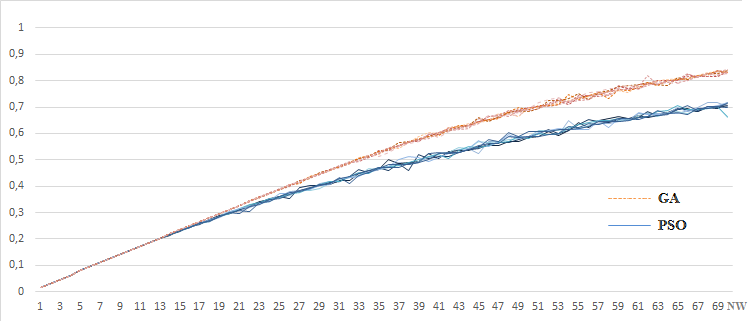
\includegraphics[width=\linewidth]{figures/GAPSObigRoomz1ters.png}
  \caption{ Comparison of  eight solution given by GA,  eight solution given by PSO algorithms with a Z equal to 1, in the big room 240x160 and ground truth equal to 64.}\label{fig:bigRz1}
   \endminipage\hfill
\end{figure}

\vfill
\hfill

\begin{figure}[!htb]
\minipage{0.62\textwidth}
  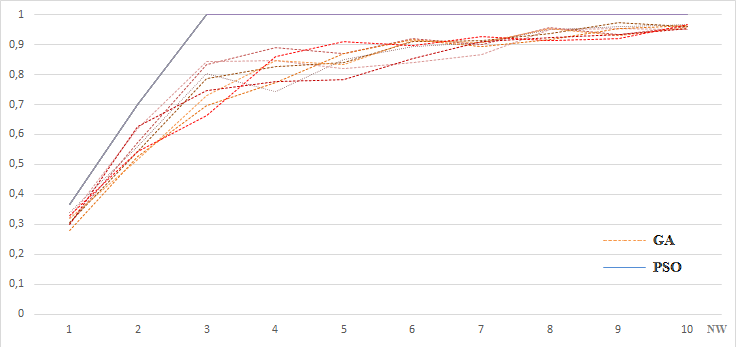
\includegraphics[width=\linewidth]{figures/GAPSORoomLz2bis.png}
  \caption{Comparison of eight solutions given by GA, eight solutions given by PSO algorithms with a Z between [1/2; 2], in the room with L shape 120x80 and ground truth equal to 15.}\label{fig:RLz2}
   \endminipage\hfill
\end{figure}

\hfill 
\vfill
\newpage

Following the comparison of the 2 algorithms, the GA seems more suited to find UAV waypoints especially if it navigates in a large room or outdoor scene. Furthermore, the comparative study demonstrated that the GA is less dependent on the shape of the  covered area. 


The number of UAV waypoints (camera pose) must be priorly known when using GA: the number of camera views is an input of the algorithm. However, in our application, it is far more interesting to assess the number of views with respect to the desired coverage rate of the area. 
To do so, a two-step procedure has been implemented. 
The first step is to find the minimum number of waypoints depending on the area to cover like  formulated in the Eq.(\ref{Eq:waypointN}). \\
\begin{equation}\label{Eq:waypointN}
\frac{ A_{room} - \sum_{i=1}^n A_{wall i} }{A_{cam}} \times \mbox{Threshold Rate} = \mbox{NWayPoint}
\end{equation}

\begin{itemize}
\item[-] $ A_{room}: $  area of the Room (length $\times$ width)
\item[-] $ A_{Wall}: $  area of the obstacle like wall (length $\times$ width)
\item[-] $ A_{Cam}: $   area cover by the camera in the maximum size of z
\item[-] $ \mbox{NWayPoint}: $  number of waypoints
\item[-] $ \mbox{Threshold Rate}: $ objective threshold rate 
\item[-] $S:$ one solution of waypoints set 
\item[-] $evalCost:$ cost function  
\end{itemize}

The second step is to compute GA optimization until the threshold is reached, while increasing the number of waypoints like explained in the algorithm \ref{alg:euclid}.  

\begin{algorithm}
\caption{}\label{alg:euclid}
\begin{algorithmic}[1]
\Procedure{N}{$a$}
 \State $S\gets 0$
  \While{$eval Cost(S)\leq ThresholdRate$}
	 \State $S \gets GA(NWayPoint)$
	  \State $NWayPoint\gets NWayPoint+1$
  \EndWhile\label{endwhile}
\State \textbf{return} $NWayPoint$
\EndProcedure
\end{algorithmic}
\end{algorithm}